%&"../net"
\endofdump
\tikzexternalize[prefix=cache/]{lab02}
\begin{document}
\title{Lab 2: Learn Mininet}
\maketitle
\tableofcontents

\section{第一题}
\subsection{题目}

Simulate the following topology in Mininet. Set the link bandwidth for (s1,s2) and (s1,s3) as 10Mbps. Use Iperf to test the TCP throughput between every host pair.

\begin{figure}[h]
    \centering
    \begin{tikzpicture}
\tikzstyle{host}=[draw]
\tikzstyle{switch}=[draw]
\tikzstyle{connection}=[]
\tikzstyle{constr}=[above,sloped,font=\ttfamily\small]
\node[host] (h1) at (-0.5,-0.5) {h1};
\node[host] (h2) at (6,-0.5) {h2};
\node[host] (h3) at (2,-4) {h3};
\node [switch] (s1) at (2,-0.5) {s1};
\node [switch] (s2) at (4,-0.5) {s2};
\node [switch] (s3) at (2,-2.5) {s3};
\draw [connection] (h1) edge (s1);
\draw [connection] (s1) edge node[constr] {10Mbps} (s2);
\draw [connection] (s2) edge (h2);
\draw [connection] (s1) edge node[constr] {10Mbps}  (s3);
\draw [connection] (s3) edge (h3);
\end{tikzpicture}
\end{figure}

第一题限制了交换机之间的带宽为 10 Mbps。

\subsection{源代码}

\code{task1.py}

\subsection{测试结果}

\begin{figure}[h]
    \centering
    \begin{multicols}{2}
    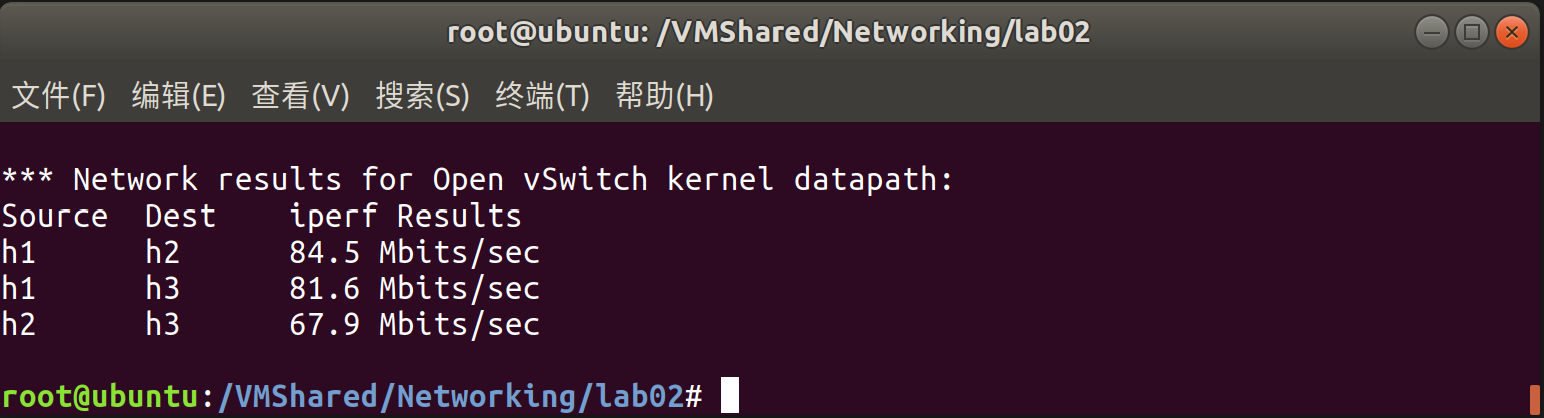
\includegraphics[width=\linewidth]{task1}

    \pgfplotstabletypeset[columns/Pair/.style={string type}]{fig/task2result.dat}
    \begin{tikzpicture}
        \begin{axis}[ymin={0},
        ylabel={TCP throughput (Mbps)},
        xlabel={host pair},
        ymax={10},
        symbolic x coords={h1-h2,h1-h3,h2-h3}, xtick=data,
        ybar,]
         \addplot+ [] table[x=Pair] {fig/task1result.dat};
        \end{axis}
        \end{tikzpicture}        
    \end{multicols}
\end{figure}

所有的对的吞吐量都被降低到了 10 Mbps 以下。

\section{第二题}

\subsection{题目}

Now let us set the packet loss rate of the link (s1,s2) and (s1,s3) as 5\%. Use Iperf to test the TCP throughput again.

\begin{figure}[h]
    \centering
    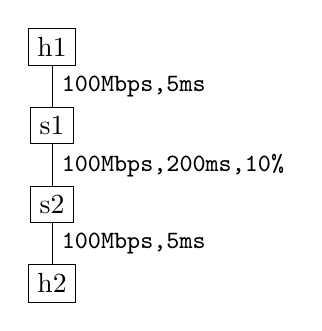
\begin{tikzpicture}
    \tikzstyle{host}=[draw]
    \tikzstyle{switch}=[draw]
    \tikzstyle{connection}=[]
    \tikzstyle{constr}=[right,font=\ttfamily\small]
    \node [host] (h1) at (0,4) {h1};
    \node [switch] (s1) at (0,3) {s1};
    \node [switch] (s2) at (0,2) {s2};
    \node [host] (h2) at (0,1) {h2};
    \draw (h1) edge node [constr] {100Mbps,5ms} (s1);
    \draw (s1) edge node [constr] {100Mbps,200ms,10\%} (s2);
    \draw (s2) edge node [constr] {100Mbps,5ms} (h2);
\end{tikzpicture}
\end{figure}

交换机之间的带宽限制为 10 Mbps,丢包率为 5\%。

\subsection{源代码变更}

\code[firstline=23,lastline=25,firstnumber=23]{task2.py}

\subsection{测试结果}

\begin{figure}[h]
    \centering
    \begin{multicols}{2}
    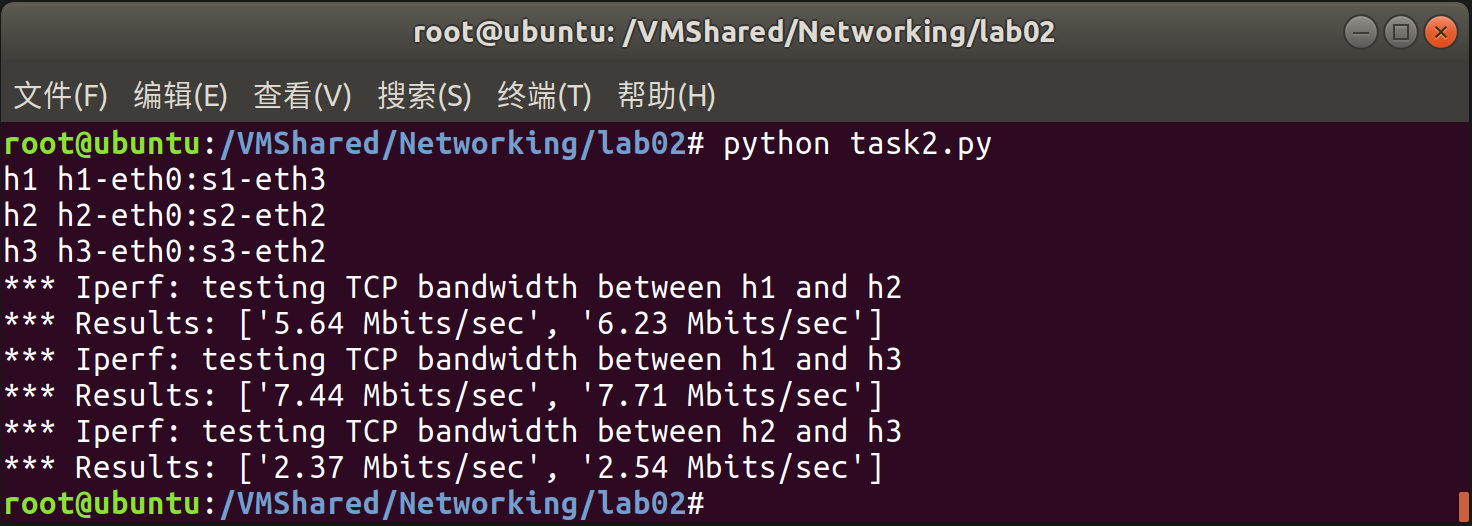
\includegraphics[width=\linewidth]{task2}

    \pgfplotstabletypeset[columns/Pair/.style={string type}]{fig/task1result.dat}
    \begin{tikzpicture}
        \begin{axis}[ymin={0},
        ylabel={TCP throughput (Mbps)},
        xlabel={host pair},
        ymax={10},
        symbolic x coords={h1-h2,h1-h3,h2-h3}, xtick=data,
        ybar,]
        \addplot+ [] table[x=Pair] {fig/task2result.dat};
        \end{axis}
        \end{tikzpicture}        
    \end{multicols}
\end{figure}

所有对的吞吐量大幅下降,其中 h2 和 h3 之间的吞吐量最低,因为会经过两个丢包链路,所以会丢失更多的包。

\section{第三题}

\subsection{题目}

Let us add another link between s2 and s3. 
Try pinging h2 from h1. What would happen?
How would you solve the problem? 
(Hint: Use ovs-ofctl command to add flow rules. )

\begin{figure}[h]
    \centering
    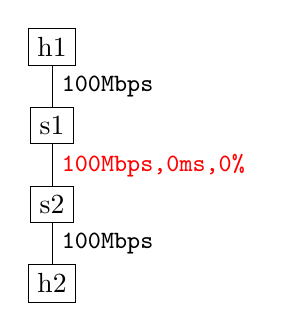
\begin{tikzpicture}
    \tikzstyle{host}=[draw]
    \tikzstyle{switch}=[draw]
    \tikzstyle{connection}=[]
    \tikzstyle{constr}=[right,font=\ttfamily\small]
    \node [host] (h1) at (0,4) {h1};
    \node [switch] (s1) at (0,3) {s1};
    \node [switch] (s2) at (0,2) {s2};
    \node [host] (h2) at (0,1) {h2};
    \draw (h1) edge node [constr] {100Mbps} (s1);
    \draw (s1) edge node [constr] {\color{red} 100Mbps,0ms,0\%} (s2);
    \draw (s2) edge node [constr] {100Mbps} (h2);
\end{tikzpicture}
\end{figure}

\subsection{源代码变更(一)}

\code[firstline=29,firstnumber=29]{task3a.py}

\subsection{测试结果(一)}

\begin{figure}[h]
    \centering
    \begin{multicols}{2}
        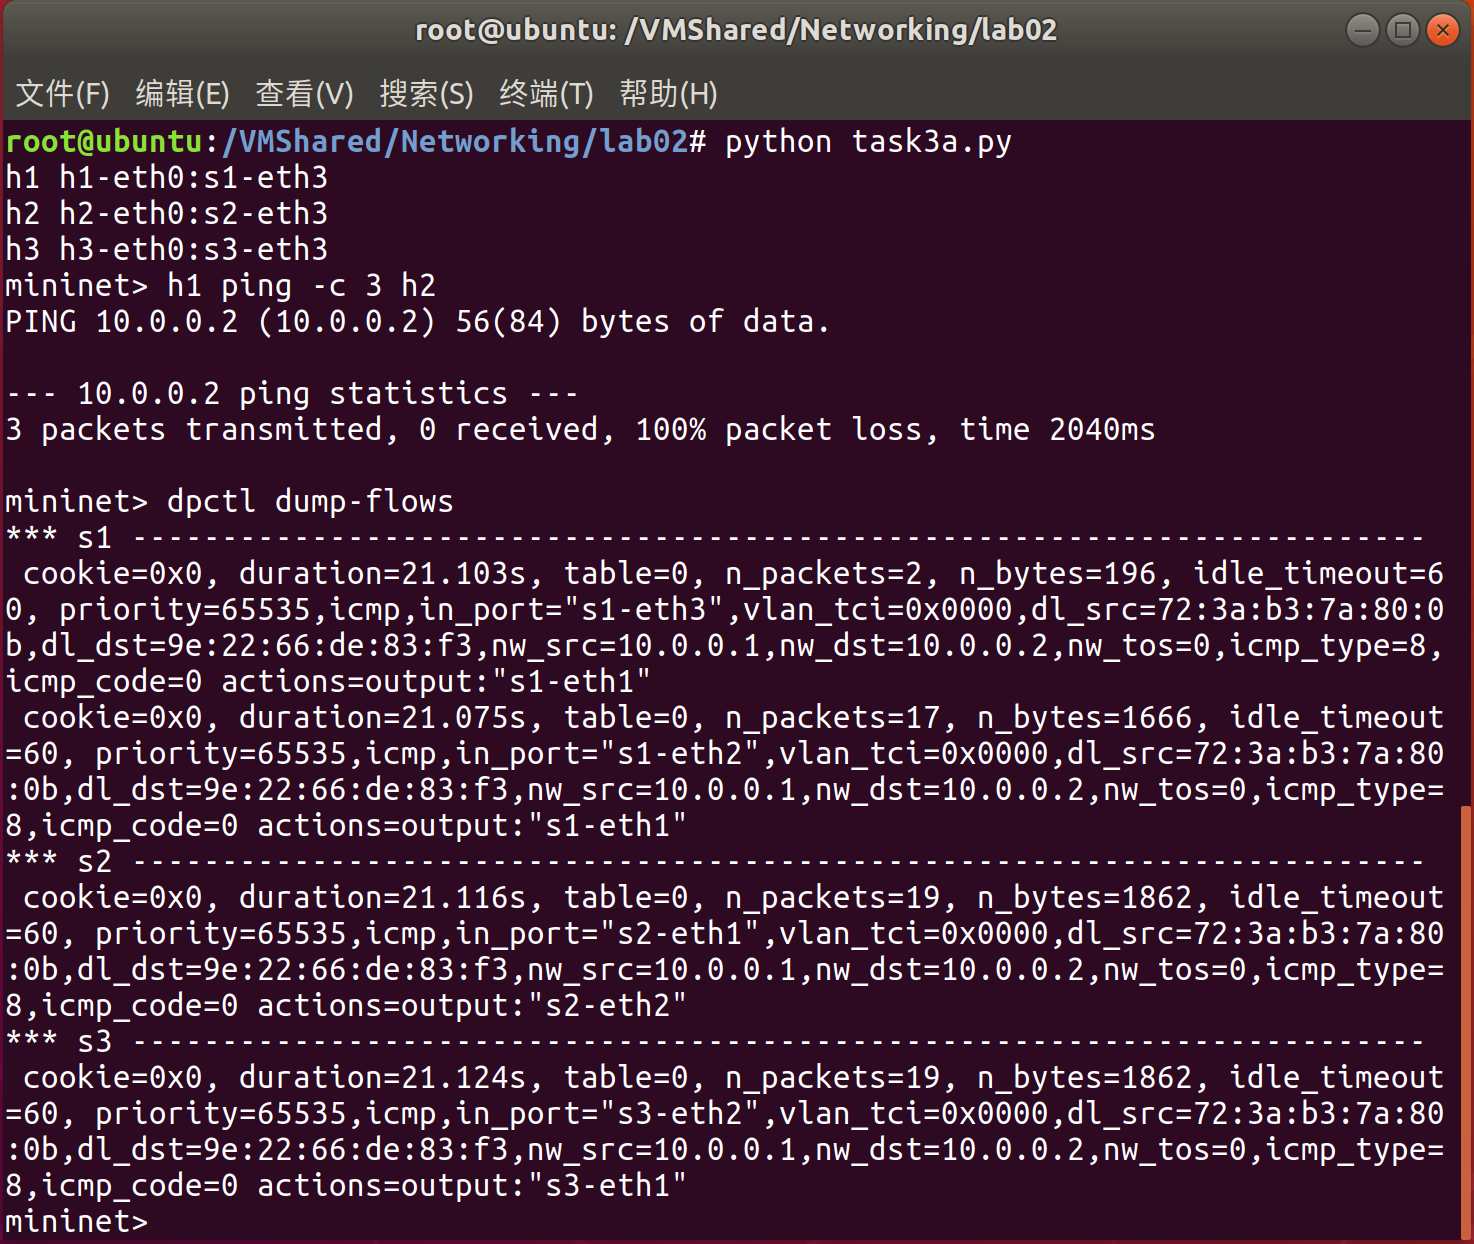
\includegraphics[width=\linewidth]{task3adump}
        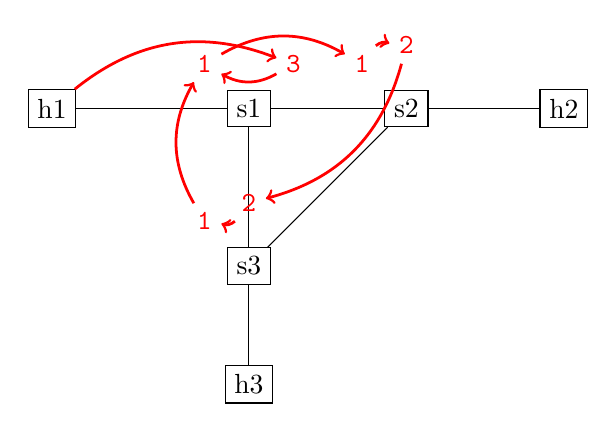
\begin{tikzpicture}[node distance=0.8cm]
\tikzstyle{host}=[draw]
\tikzstyle{switch}=[draw]
\tikzstyle{connection}=[]
\tikzstyle{constr}=[above,sloped,font=\ttfamily\small]
\tikzstyle{moreconstr} = [constr,below]
\tikzstyle{port}=[red,font=\ttfamily]
\tikzstyle{passing}=[->,bend left, line width=1pt,red]
\node[host] (h1) at (-0.5,-0.5) {h1};
\node[host] (h2) at (6,-0.5) {h2};
\node[host] (h3) at (2,-4) {h3};
\node [switch] (s1) at (2,-0.5) {s1};
\node [switch] (s2) at (4,-0.5) {s2};
\node [switch] (s3) at (2,-2.5) {s3};
\draw [connection] (h1) edge (s1);
\draw [connection] (s1) edge (s2);
\draw [connection] (s2) edge (h2);
\draw [connection] (s1) edge (s3);
\draw [connection] (s3) edge (h3);
\draw [connection] (s2) edge (s3);
\node [above left of=s1,port] (s1p1) {1};
\node [above right of=s1,port] (s1p3) {3};
\node [above left of=s2,port] (s2p1) {1};
\node [above of=s2,port] (s2p2) {2};
\node [above left of=s3,port] (s3p1) {1};
\node [above of=s3,port] (s3p2) {2};

\draw [passing] (h1) edge (s1p3);
\draw [passing] (s1p3) edge (s1p1);
\draw [passing] (s1p1) edge (s2p1);
\draw [passing] (s2p1) edge (s2p2);
\draw [passing] (s2p2) edge (s3p2);
\draw [passing] (s3p2) edge (s3p1);
\draw [passing] (s3p1) edge (s1p1);
\end{tikzpicture}
    \end{multicols}
\end{figure}

测试显示 h1 到 h2 的包全部丢失。图中还显示了流表信息。右图展示了一个从 h1 发出的包会导致端口间转发循环的一种情况,在这种默认的配置下,会导致找不到到达 h2 的通路。

\subsection{源代码变更(二)}

\code[firstline=29,firstnumber=29]{task3b.py}

\subsection{测试结果(二)}

\begin{figure}[h]
    \centering
    \begin{multicols}{2}
        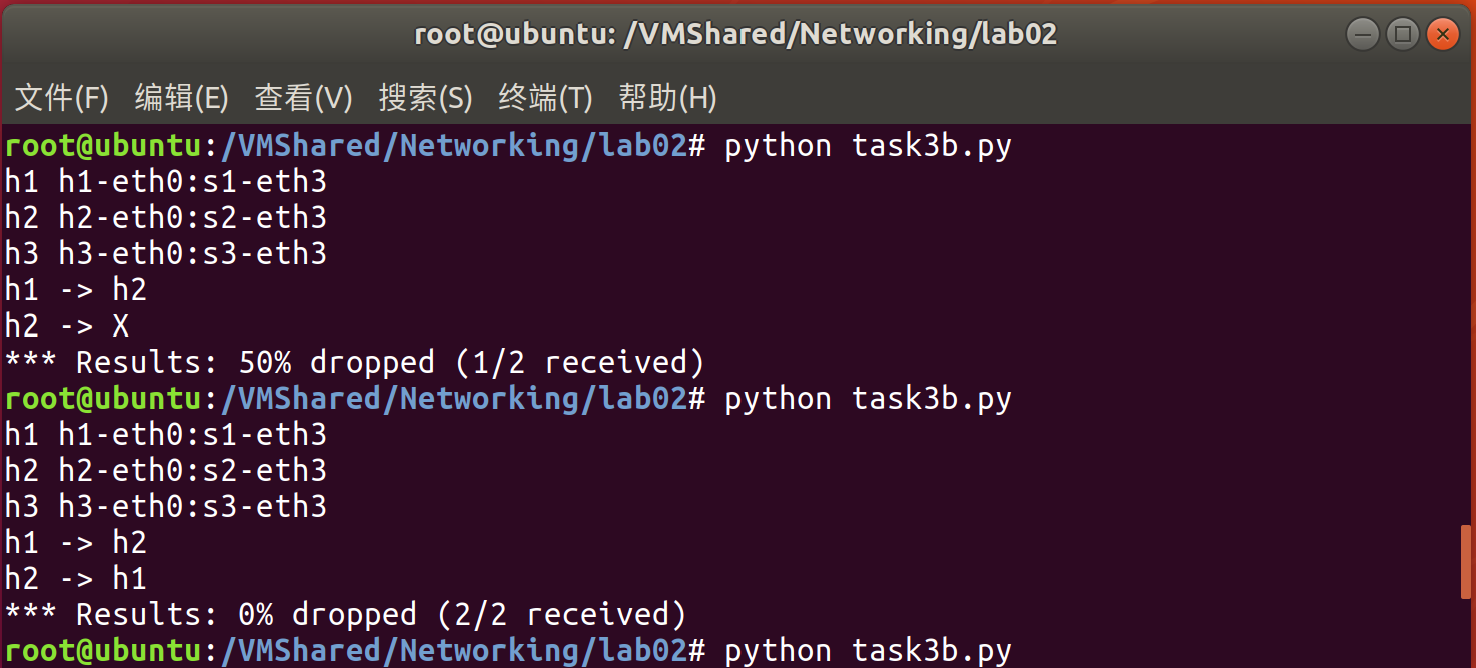
\includegraphics[width=\linewidth]{task3b}
        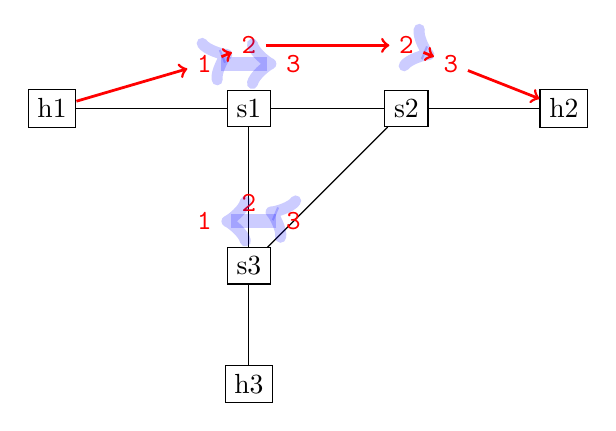
\begin{tikzpicture}[node distance=0.8cm]
\tikzstyle{host}=[draw]
\tikzstyle{switch}=[draw]
\tikzstyle{connection}=[]
\tikzstyle{constr}=[above,sloped,font=\ttfamily\small]
\tikzstyle{moreconstr} = [constr,below]
\tikzstyle{port}=[red,font=\ttfamily]
\tikzstyle{passing}=[->,bend left, line width=1pt,red]
\tikzstyle{send}=[->,line width=5pt,blue,opacity=0.2]
\node[host] (h1) at (-0.5,-0.5) {h1};
\node[host] (h2) at (6,-0.5) {h2};
\node[host] (h3) at (2,-4) {h3};
\node [switch] (s1) at (2,-0.5) {s1};
\node [switch] (s2) at (4,-0.5) {s2};
\node [switch] (s3) at (2,-2.5) {s3};
\draw [connection] (h1) edge (s1);
\draw [connection] (s1) edge (s2);
\draw [connection] (s2) edge (h2);
\draw [connection] (s1) edge (s3);
\draw [connection] (s3) edge (h3);
\draw [connection] (s2) edge (s3);
\node [above left of=s1,port] (s1p1) {1};
\node [above of=s1,port] (s1p2) {2};
\node [above right of=s1,port] (s1p3) {3};
\node [above of=s2,port] (s2p2) {2};
\node [above right of=s2,port] (s2p3) {3};
\node [above left of=s3,port] (s3p1) {1};
\node [above of=s3,port] (s3p2) {2};
\node [above right of=s3,port] (s3p3) {3};

\draw[send] (s1p1) -- (s1p2);
\draw[send] (s1p1) -- (s1p3);
\draw[send] (s2p2) -- (s2p3);
\draw[send] (s3p3) -- (s3p1);
\draw[send] (s3p3) -- (s3p2);

\draw[passing] (h1) -- (s1p1);
\draw[passing] (s1p1) -- (s1p2);
\draw[passing] (s1p2) -- (s2p2);
\draw[passing] (s2p2) -- (s2p3);
\draw[passing] (s2p3) -- (h2);

\end{tikzpicture}
    \end{multicols}
\end{figure}

通过手动添加流表规则,
\begin{quotation}
    \noindent s1p1$\rightarrow$s1p2,s1p3\\
    s2p2$\rightarrow$s2p3\\
    s3p3$\rightarrow$s3p1,s3p2
\end{quotation}
就能够实现 h1 到 h2 的通信。

\end{document}